\documentclass[../competing_bandits.tex]{subfiles}
\begin{document}

\section{Algorithms' Performance in Isolation: Revisited}\label{section:revisited}

Conjecture~\ref{conj:inverted-u} for the most part is validated by our simulation results, but Puzzles~\ref{puz:dg_ht} and \ref{puz:nih} seem to be problematic for it.

We first attempt to explain Puzzle~\ref{puz:dg_ht} by revisiting Conjecture~\ref{conj:mean-trajectories}.

\begin{finding}
\textit{
Conjecture~\ref{conj:mean-trajectories} is false. Mean reputation trajectories do not suffice to explain the outcomes under competition.}
\end{finding}

\begin{figure}[ht]
\caption{Distribution of reputation scores for Needle-in-Haystack at $t=500$ (smoothed using a kernel density estimate)}
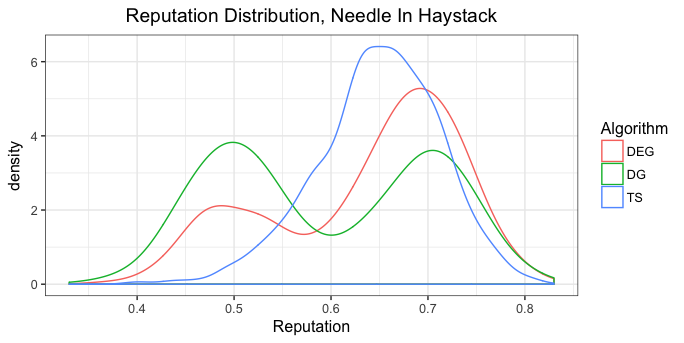
\includegraphics[scale=0.35]{figures/rep_distribution_nih}
\label{rep_dist_nih}
%\caption*{\tiny{The plots contain a kernel density estimate of the reputation distribution at $t = 500$}}
\end{figure}

To see what could go wrong, consider how an algorithm's reputation score is distributed at a particular time. That is, consider the empirical distribution of this score over different \MRVs. For concreteness, we consider the needle-in-haystack instance at time $t=500$ (Figure \ref{rep_dist_nih}) since the intuition as to why the mean may be misleading is clearest on this instance (though the same result holds across the instances).

We see that the ``naive" algorithms $\DG$ and $\DEG$ have a bi-modal reputation distribution, whereas $\TS$ does not. The reason is that for this MAB instance, $\DG$ either finds the best arm and sticks to it, or gets stuck on the bad arms. This leads to two cases: $\DG$ either does slightly better than $\TS$ or where $\TS$ does substantially better than $\DG$.

However, the mean reputation trajectory of an algorithm would summarize all this complexity the average over the \MRVs. This may be inadequate for explaining the outcome of the duopoly game, given that the latter is determined by a simple comparison between the firm's reputation scores. Further, consider the difference in reputation scores (\emph{reputation difference}) between \TS and \DG on a particular \MRV. Let's plot the empirical distribution of the reputation difference (over the \MRVs) at a particular time point. Figure~\ref{ts_dg_rep_diff_nih} shows such plots for several time points.

We observe that the distribution is skewed to the right, precisely due to the fact that $\DG$ either does slightly better than $\TS$ or does substantially worse. This means that the mean is not a good measure of the central tendency, or typical value, of the reputation difference distribution and overstates how well an advanced exploration algorithm (that will eventually find the best arm) should do in competition compared to a naive algorithm that may never find the best arm.

\begin{figure}[ht]
\caption{Distribution of reputation difference $\TS-\DG$ for the Needle-in-Haystack (smoothed via a kernel density estimate)}
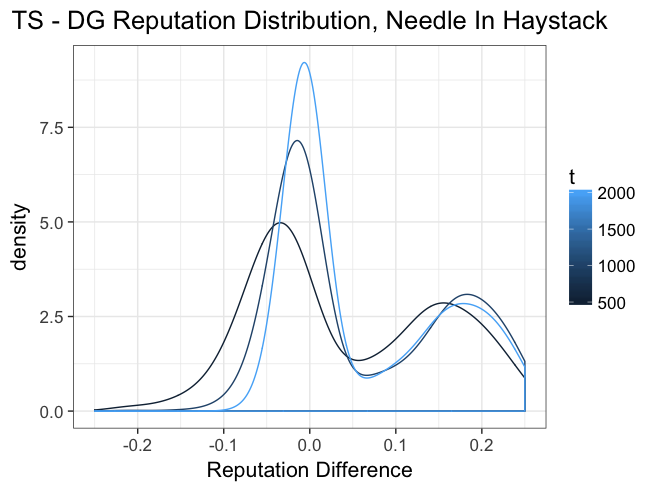
\includegraphics[scale=0.35]{figures/ts_dg_rep_diff_nih}
\label{ts_dg_rep_diff_nih}
%\caption*{\tiny{The plots contain a kernel density estimate of the difference in reputation between $\TS$ and $\DG$ across $t$}}
\end{figure}

Let us consider a statistic with a more direct connection to the competition game: for each time $t$, the proportion of \MRVs for which one algorithm has a higher reputation score than the other. 

\begin{definition}
\textit{Relative Reputation Proportion} - the proportion of simulations in which algorithm $A$ had at least as high of a reputation as algorithm $B$ for a fixed time $t$
\end{definition}


\begin{finding}
\textit{Purposeful exploration can lead to relative reputational costs compared to the greedy alternative and this leads to $\TS$ doing worse than $\DG$ for small time horizons. We observe this under the Uniform and Heavy Tail instances. However, it is not observed under the Needle In Haystack instances}
\end{finding}

The relative reputation proportion statistic corresponds to running the bandit algorithms in isolation on the same instance and with the same realizations for $t$ rounds and then calculating the fraction of simulations at which an agent would select a firm playing $A$ over a firm playing $B$ at time $t$.

\begin{figure}[ht]
\caption{Relative Reputation Proportion Plots for $\TS$ vs $\DG$. Shaded area display 95\% confidence intervals.}
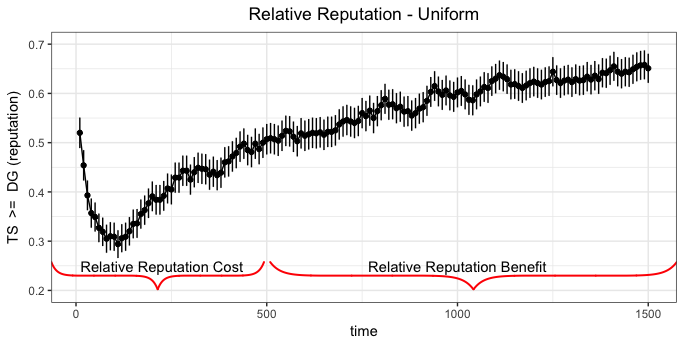
\includegraphics[scale=0.35]{figures/relative_uniform_annotated_plot}
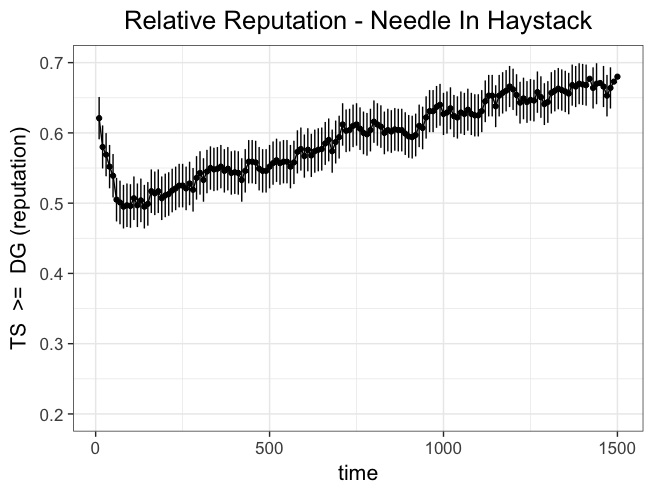
\includegraphics[scale=0.35]{figures/relative_nih_ts_dg.png}
%\caption*{\tiny{The plots contain the average reputation over $1000$ runs for a memory size of $100$ where, for a given $t$, we record the reputation of both of the algorithms on a given instance and then calculate the proportion of runs where $\TS \geq \DG$. The shaded area display 95\% confidence intervals.}}
\label{relative_rep_plots}

\end{figure}

Figure \ref{relative_rep_plots} shows plots of the relative reputation proportion for $\TS$ vs $\DG$ on the Uniform and Needle In Haystack instances. For the Uniform instance we see that, in the early rounds, the relative reputation proportion for $\TS$  vs. $\DG$ is less than 0.5 meaning that $\DG$ has a higher reputation in a majority of the simulations  but that, eventually, $\TS$ does better than $\DG$ in a majority of the simulations. The intuition behind this is that, especially since the firms start with no substantive initial information, $\TS$ does purposeful exploration in the early rounds in order to acquire information which leads to a relatively lower reputation compared to $\DG$. However, eventually the information acquired from purposeful exploration in the early rounds allows $\TS$ to make better decisions and achieve a higher reputation, especially when the instance is ``hard enough" so that $\DG$ cannot trivially find the best arm. The early exploration leads to what we define as a \textit{relative reputation cost} and the eventual gain in reputation leads to what we define as a \textit{relative reputation benefit}.

\begin{definition}
\textit{Relative reputation cost and benefit} - the relative reputation loss an algorithm incurs from purposeful exploration compared to the greedy alternative. Here we treat it as an empirical definition based on the relative reputation proportion where the ``cost" regime is when the proportion $< 0.5$ and the ``benefit" regime is when the proportion is $> 0.5$ for the better algorithm. We call the instances where there is an early costly period followed by a later benefit period relative reputation costly instances.
\end{definition}

Is exploration always costly? Figure \ref{relative_rep_plots} also shows that for the Needle In Haystack instances, $\TS$ always does relatively better than $\DG$. There are two contributing factors to this. First, $\TS$ identifies the best arm faster in the Needle In Haystack instances than the Uniform instances so that there is a shorter time horizon where $\TS$ needs to engage in purposeful exploration. Second, in the Needle In Haystack instances there are no ``bad" arms as there may be in the Uniform instances since by construction all the arms except one in Needle In Haystack are the same. Thus, when $\TS$ pulls a sub-optimal arm relative to its current information, the expected reward is the same as the greedy option that has not identified the best arm. However, with the Uniform instances, it is possible that the sub-optimal arm that is pulled has substantially lower expected reward relative to the greedy option. Thus, only the Uniform and Heavy Tail instances are relative reputation costly instances.

This observation allows us to explain the Puzzle~\ref{puz:nih} from the competition game and establish a more nuanced view of the inverted-U.

\begin{finding}
\textit{For sufficiently low warm start \emph{under the instances that are relative reputation costly}, the optimal strategies in the competition game are:
\begin{center}
\textbf{Permanent Monopoly} - $DG$ \\
\textbf{Temporary Monopoly} - $\TS$ \\
\textbf{Permanent Duopoly} - $DG$ \\
\end{center}
The conditions on $\TS$ being dominant under the temporary monopoly are that the incumbent is a temporary monopoly for sufficiently many periods.
}
\end{finding}

Thus, the reason we see that $\DG$ is better than $\TS$ under Heavy Tail and Uniform but that $\TS$ is always preferred under Needle In Haystack is due to the fact that the purposeful exploration engaged by $\TS$ in the early rounds leads it to suffer a relative reputational cost in the former case but not in the latter. Looking at the relative reputation plots in Figure \ref{relative_rep_plots}, we can interpret fixing a warm start $T_0$ as fixing the starting point on the relative reputation plots. The proportion of first rounds in the competition game that will go to a firm playing alg $A$ over a firm playing alg $B$ will correspond to the relative reputation proportion at time $T_0$. As a result, if we begin with a warm start that falls in the region where the proportion $< 0.5$, we expect that $\DG$ does better than $\TS$.

This also allows us to give some intuition as to why allowing one firm to be a temporary monopoly incentivizes it to play $\TS$ even if, for the same warm start, the firm would be incentivized to play $\DG$ under permanent duopoly.  By allowing it to be the only firm in the market for sufficiently long we allow it to recoup the reputation costs by having it engage in most of its exploration while it does not have the pressure to incentivize agents to select them over their competition.


\end{document} 